\section{Experimentdesign}

Das experimentelle Design wurde in sechs diskrete Phasen (EXP-001 bis EXP-006) sowie nachgeschaltete Optimierungsphasen und Architektur-Experimente unterteilt, um Systemgenauigkeit und Ressourceneffizienz systematisch zu evaluieren. Die Experimente gliedern sich in Stage~A (Klassifikation) und Stage~B (Detektion), wobei Stage~B eine Migration der Basisarchitektur von YOLOv8-Nano zu YOLO11n umfasst.

\subsection{Klassifikationsphase (EXP-001 bis EXP-004)}
Die erste Phase verglich drei Architekturen auf demselben Validierungssplit: ein Scratch-CNN (EXP-001, Val.~Accuracy~\SI{61.00}{\percent}), MobileNetV2 mit gefrorenem Backbone (EXP-002, \SI{84.28}{\percent}) und MobileNetV2 mit Fine-Tuning (EXP-003, \SI{87.42}{\percent}). Ziel war zu prüfen, wie stark Transfer Learning den Sprung von einem kleinen, direkt trainierten Netz zu einem robusteren Modell verbessert \cite{yosinski2014transferable}.

\begin{figure}[H]
    \centering
    \begin{subfigure}[b]{0.31\textwidth}
        \centering
        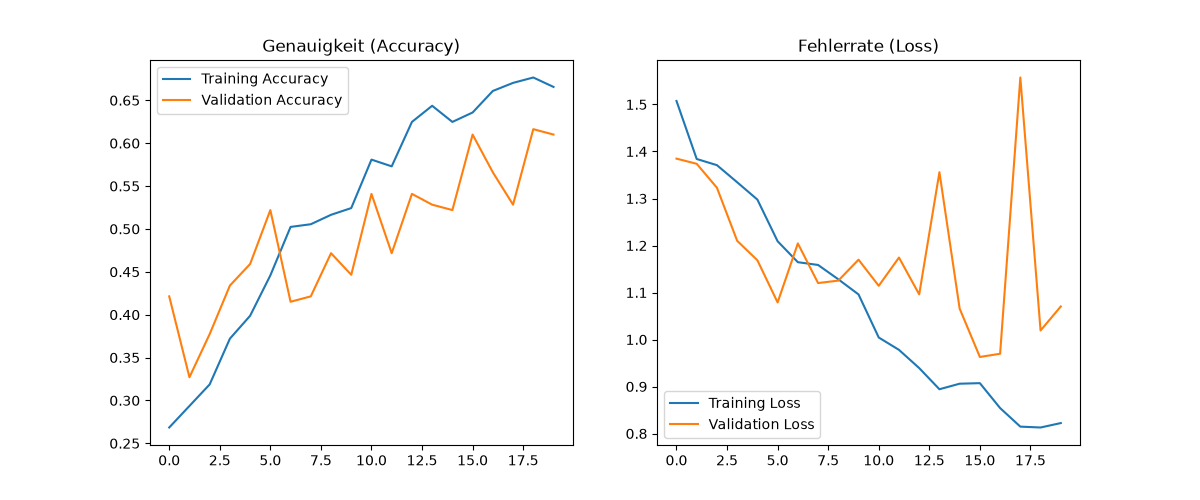
\includegraphics[width=\textwidth, keepaspectratio]{figures/exp1-curves.png}
        \caption{EXP-001 (CNN)}
    \end{subfigure}
    \hfill
    \begin{subfigure}[b]{0.31\textwidth}
        \centering
        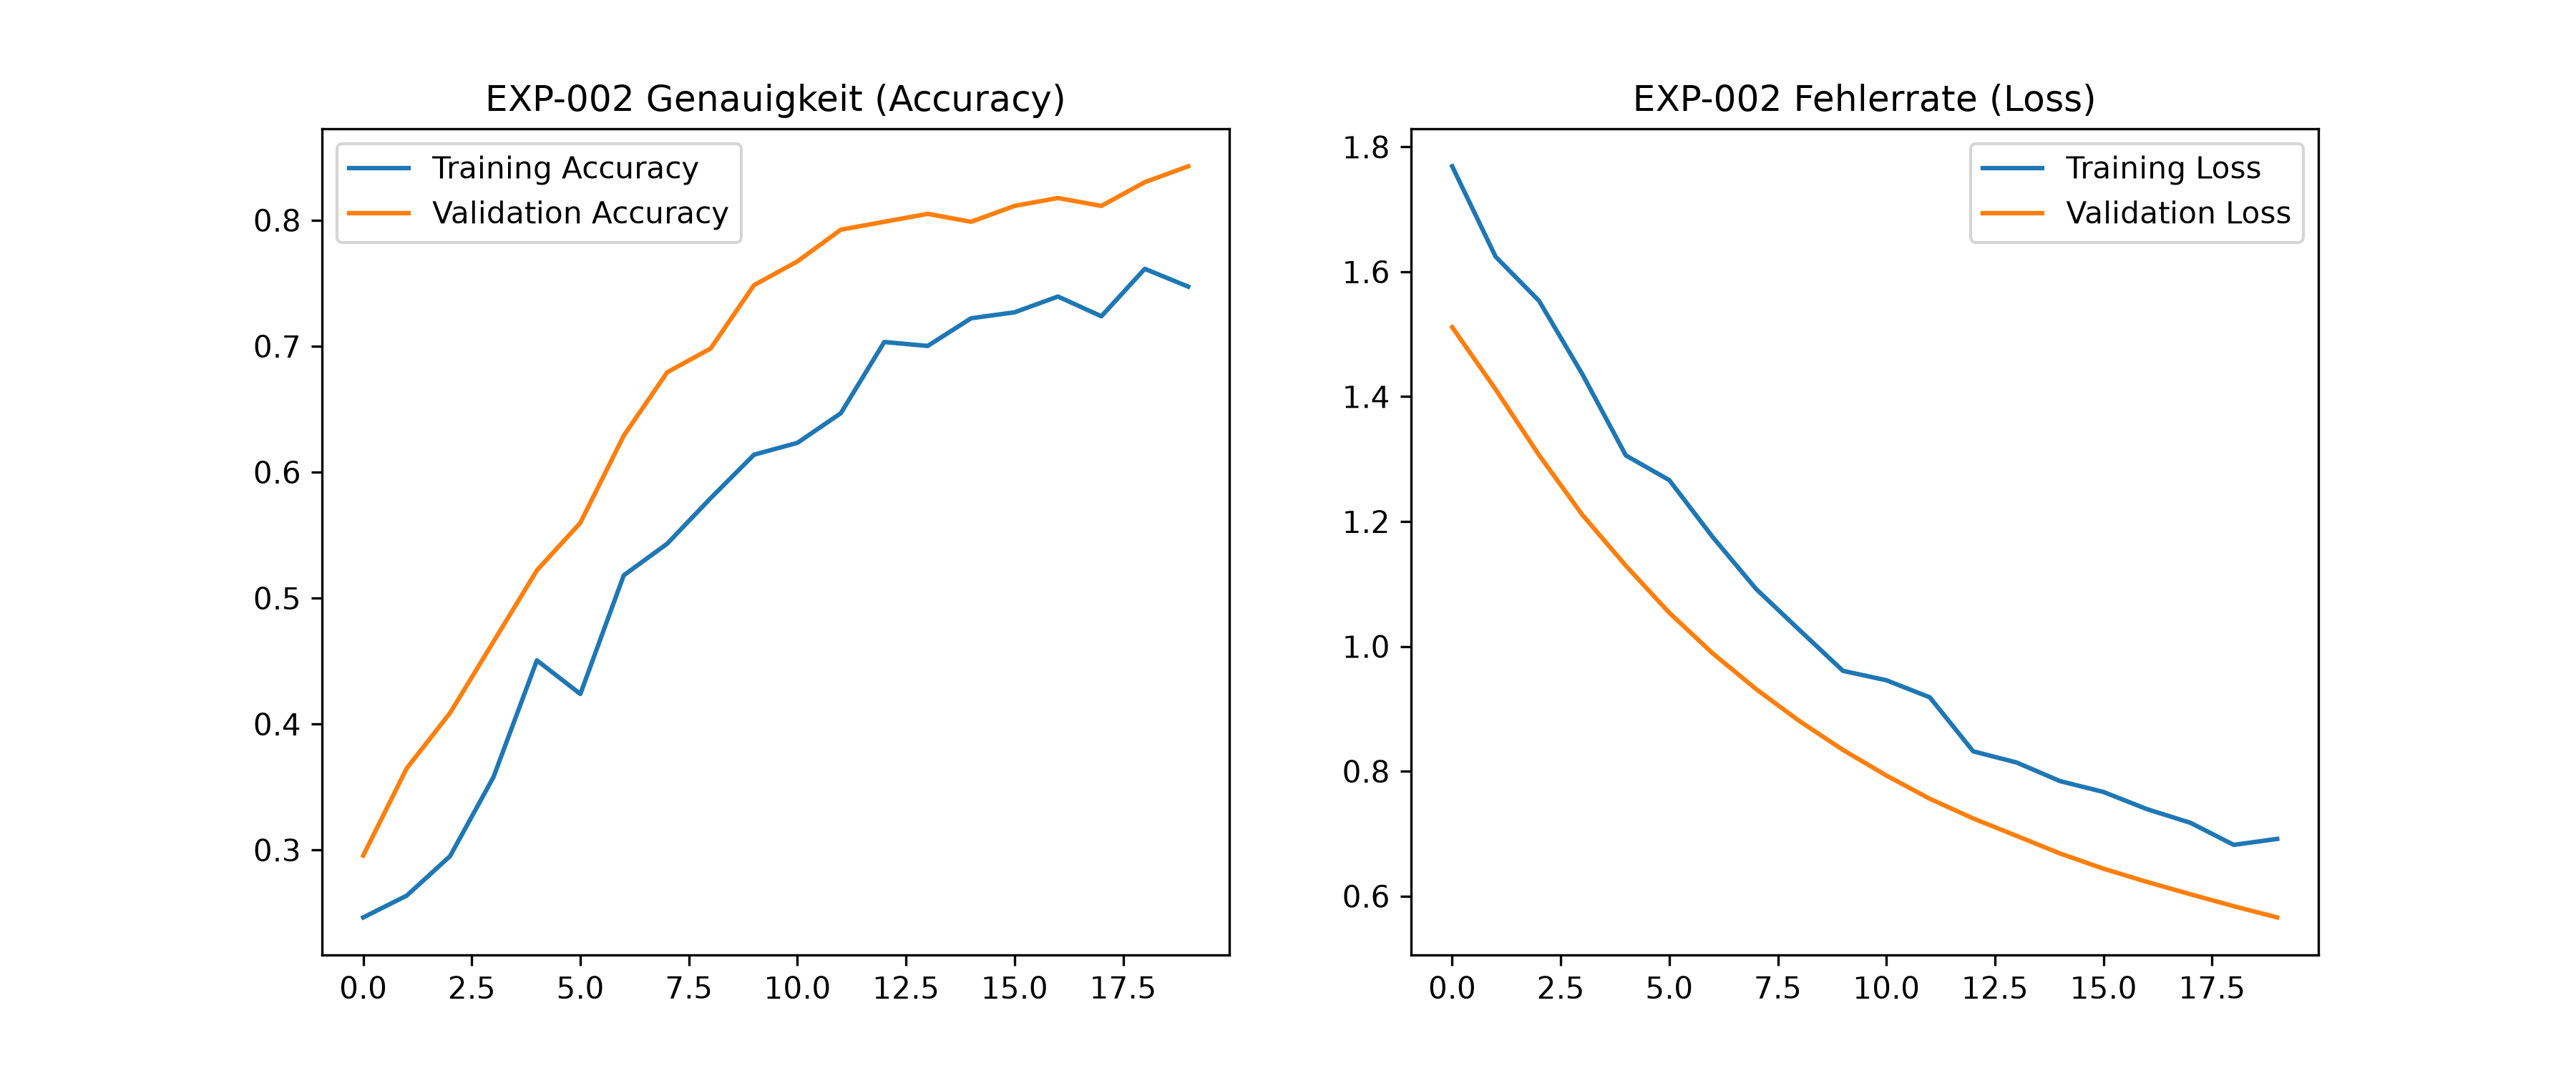
\includegraphics[width=\textwidth, keepaspectratio]{figures/exp2-curves.png}
        \caption{EXP-002 (Frozen)}
    \end{subfigure}
    \hfill
    \begin{subfigure}[b]{0.31\textwidth}
        \centering
        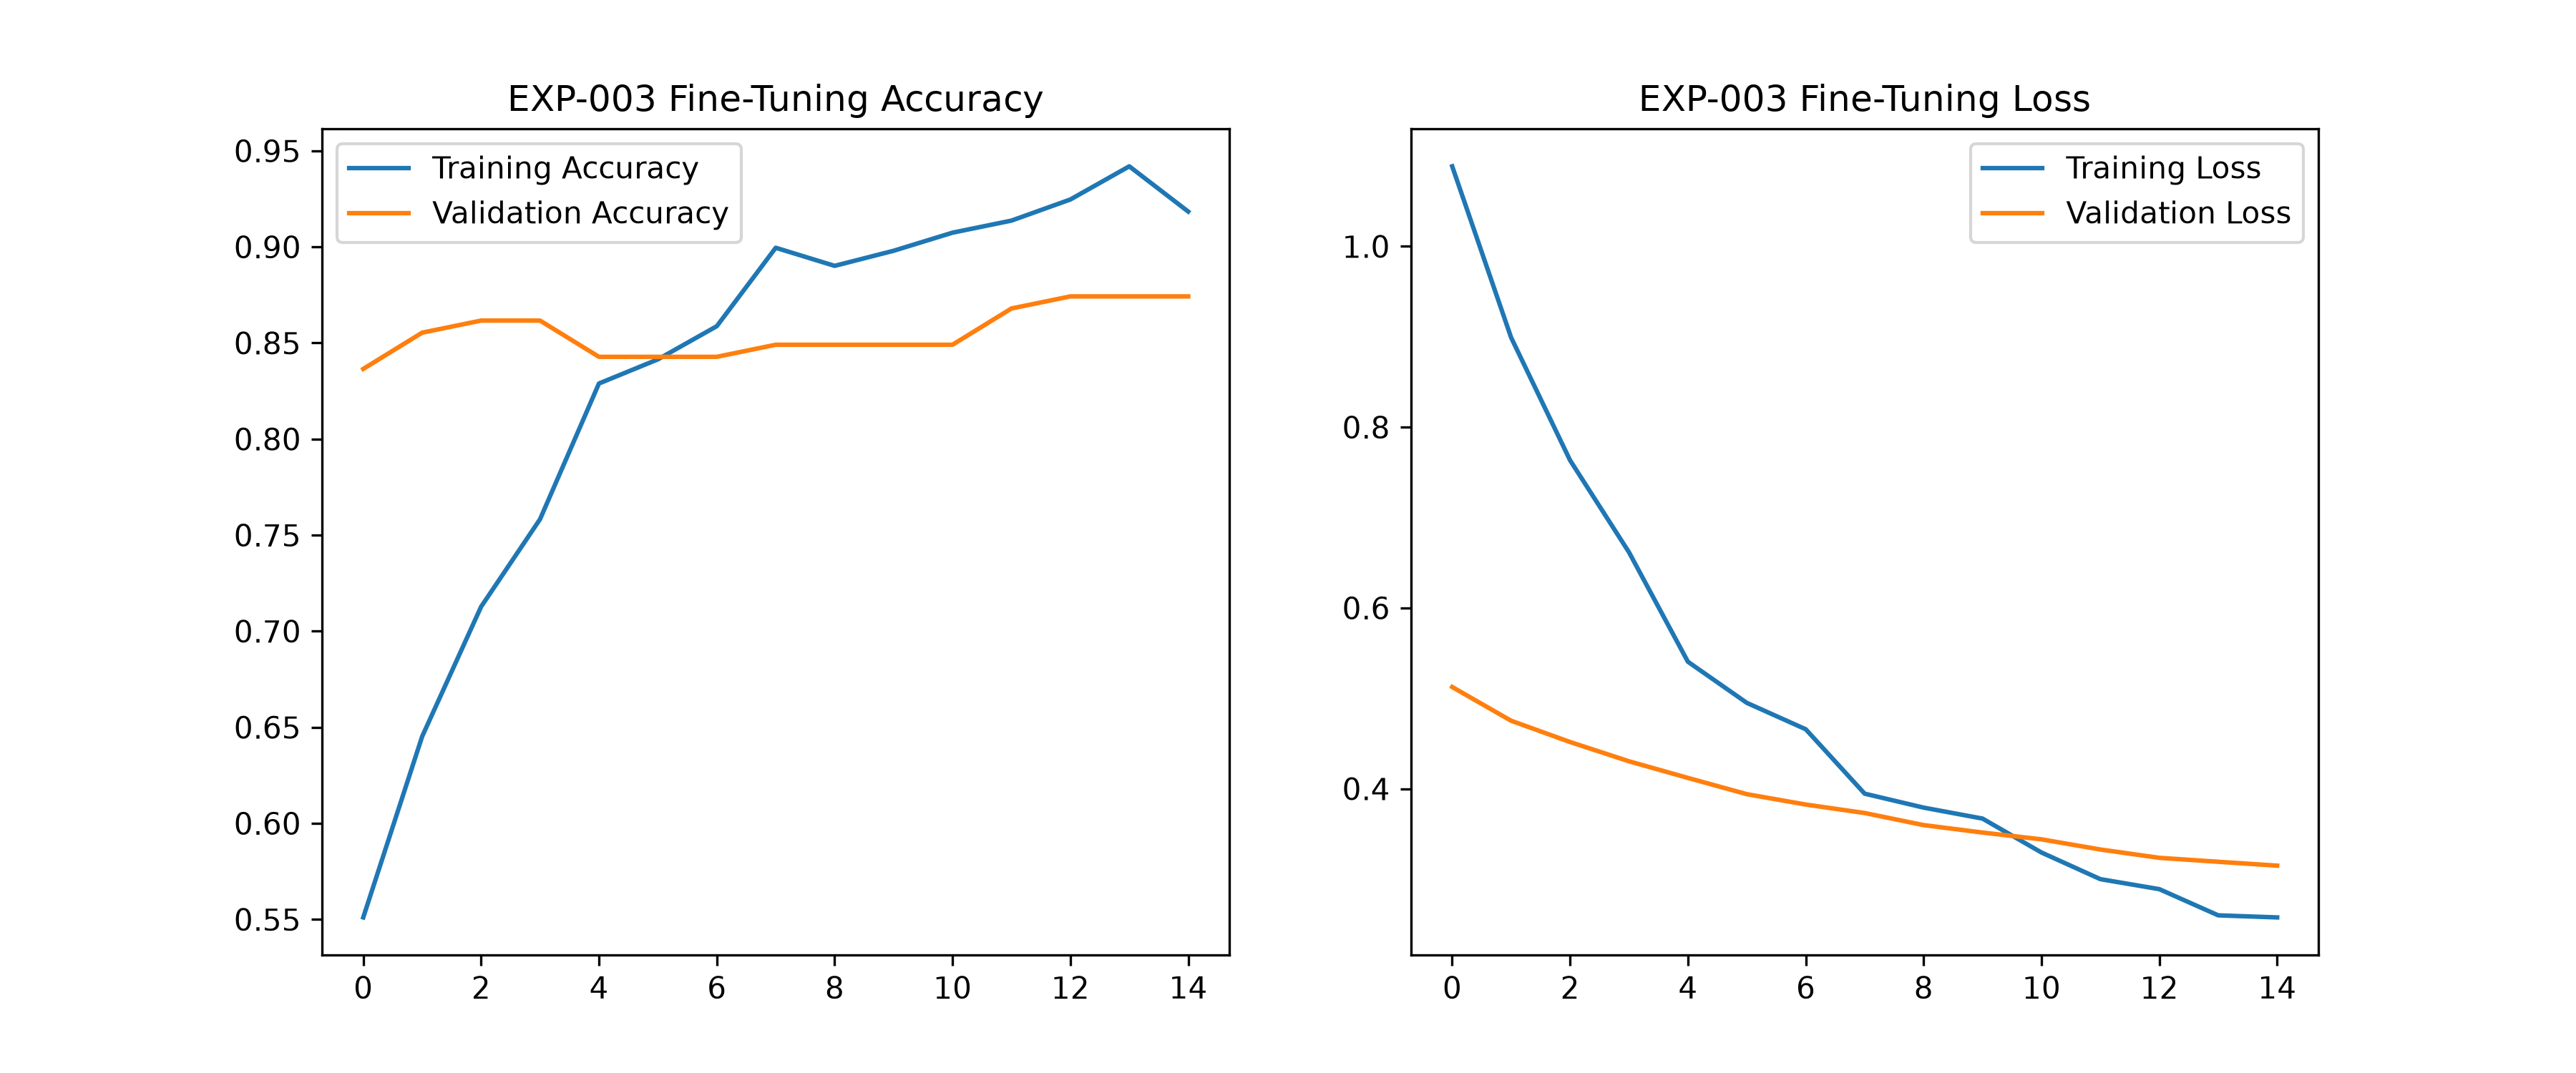
\includegraphics[width=\textwidth, keepaspectratio]{figures/exp3-curves.png}
        \caption{EXP-003 (Fine-Tune)}
    \end{subfigure}
    \caption{Trainings- und Validierungskurven (Accuracy/Loss über Epochen) der drei Klassifikationsmodelle. EXP-001 zeigt starkes Rauschen; EXP-003 konvergiert am stabilsten.}
    \label{fig:curves-class}
\end{figure}

\begin{figure}[H]
    \centering
    \begin{subfigure}[b]{0.31\textwidth}
        \centering
        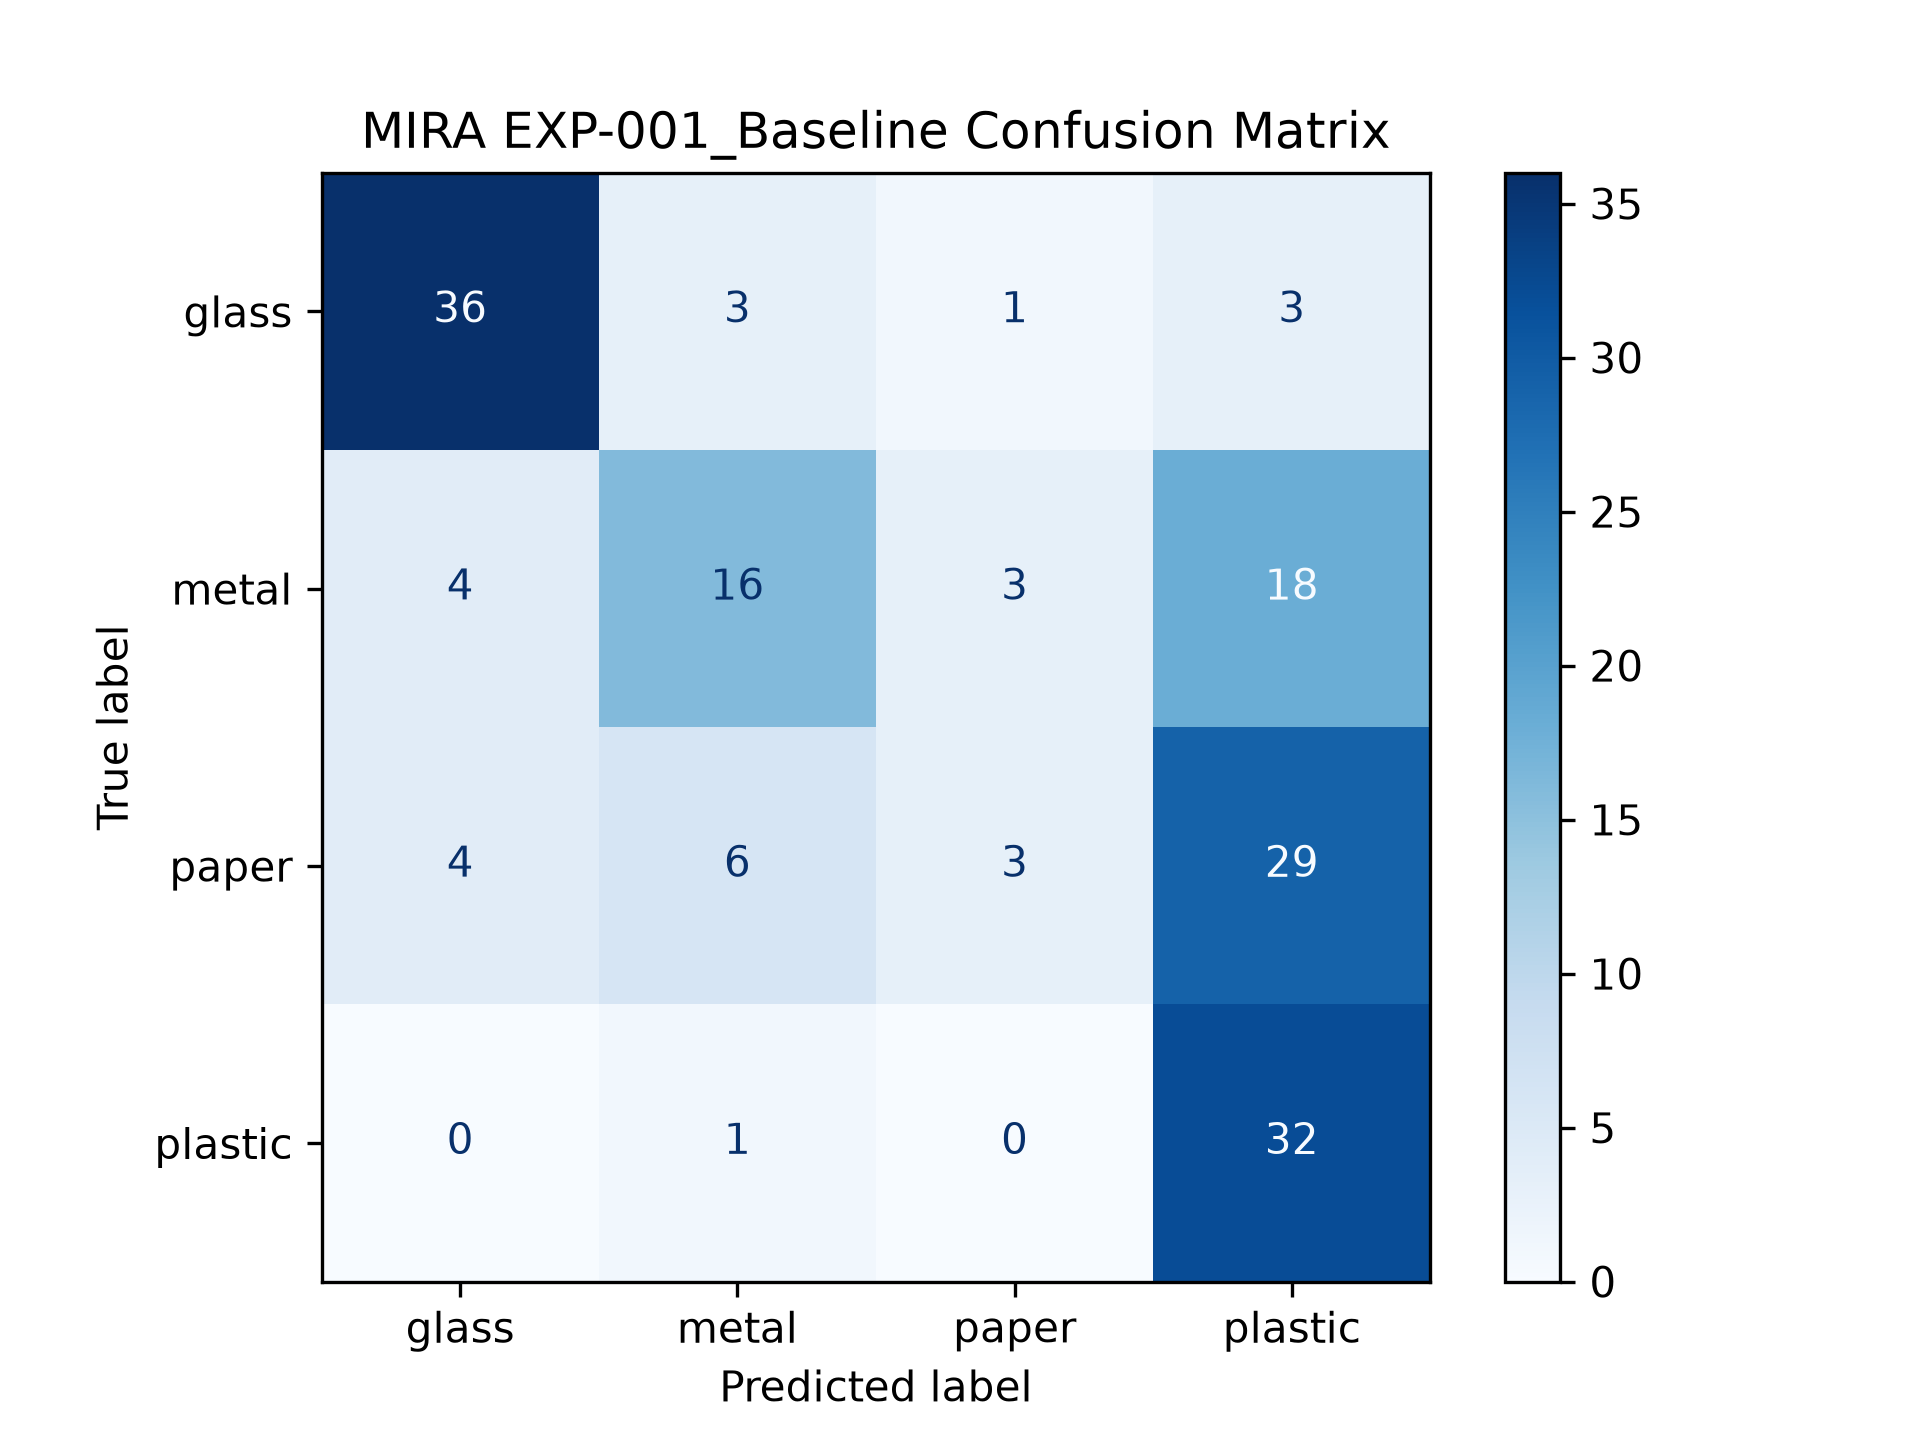
\includegraphics[width=\textwidth, keepaspectratio]{figures/exp1-confusion.png}
        \caption{EXP-001 (CNN)}
    \end{subfigure}
    \hfill
    \begin{subfigure}[b]{0.31\textwidth}
        \centering
        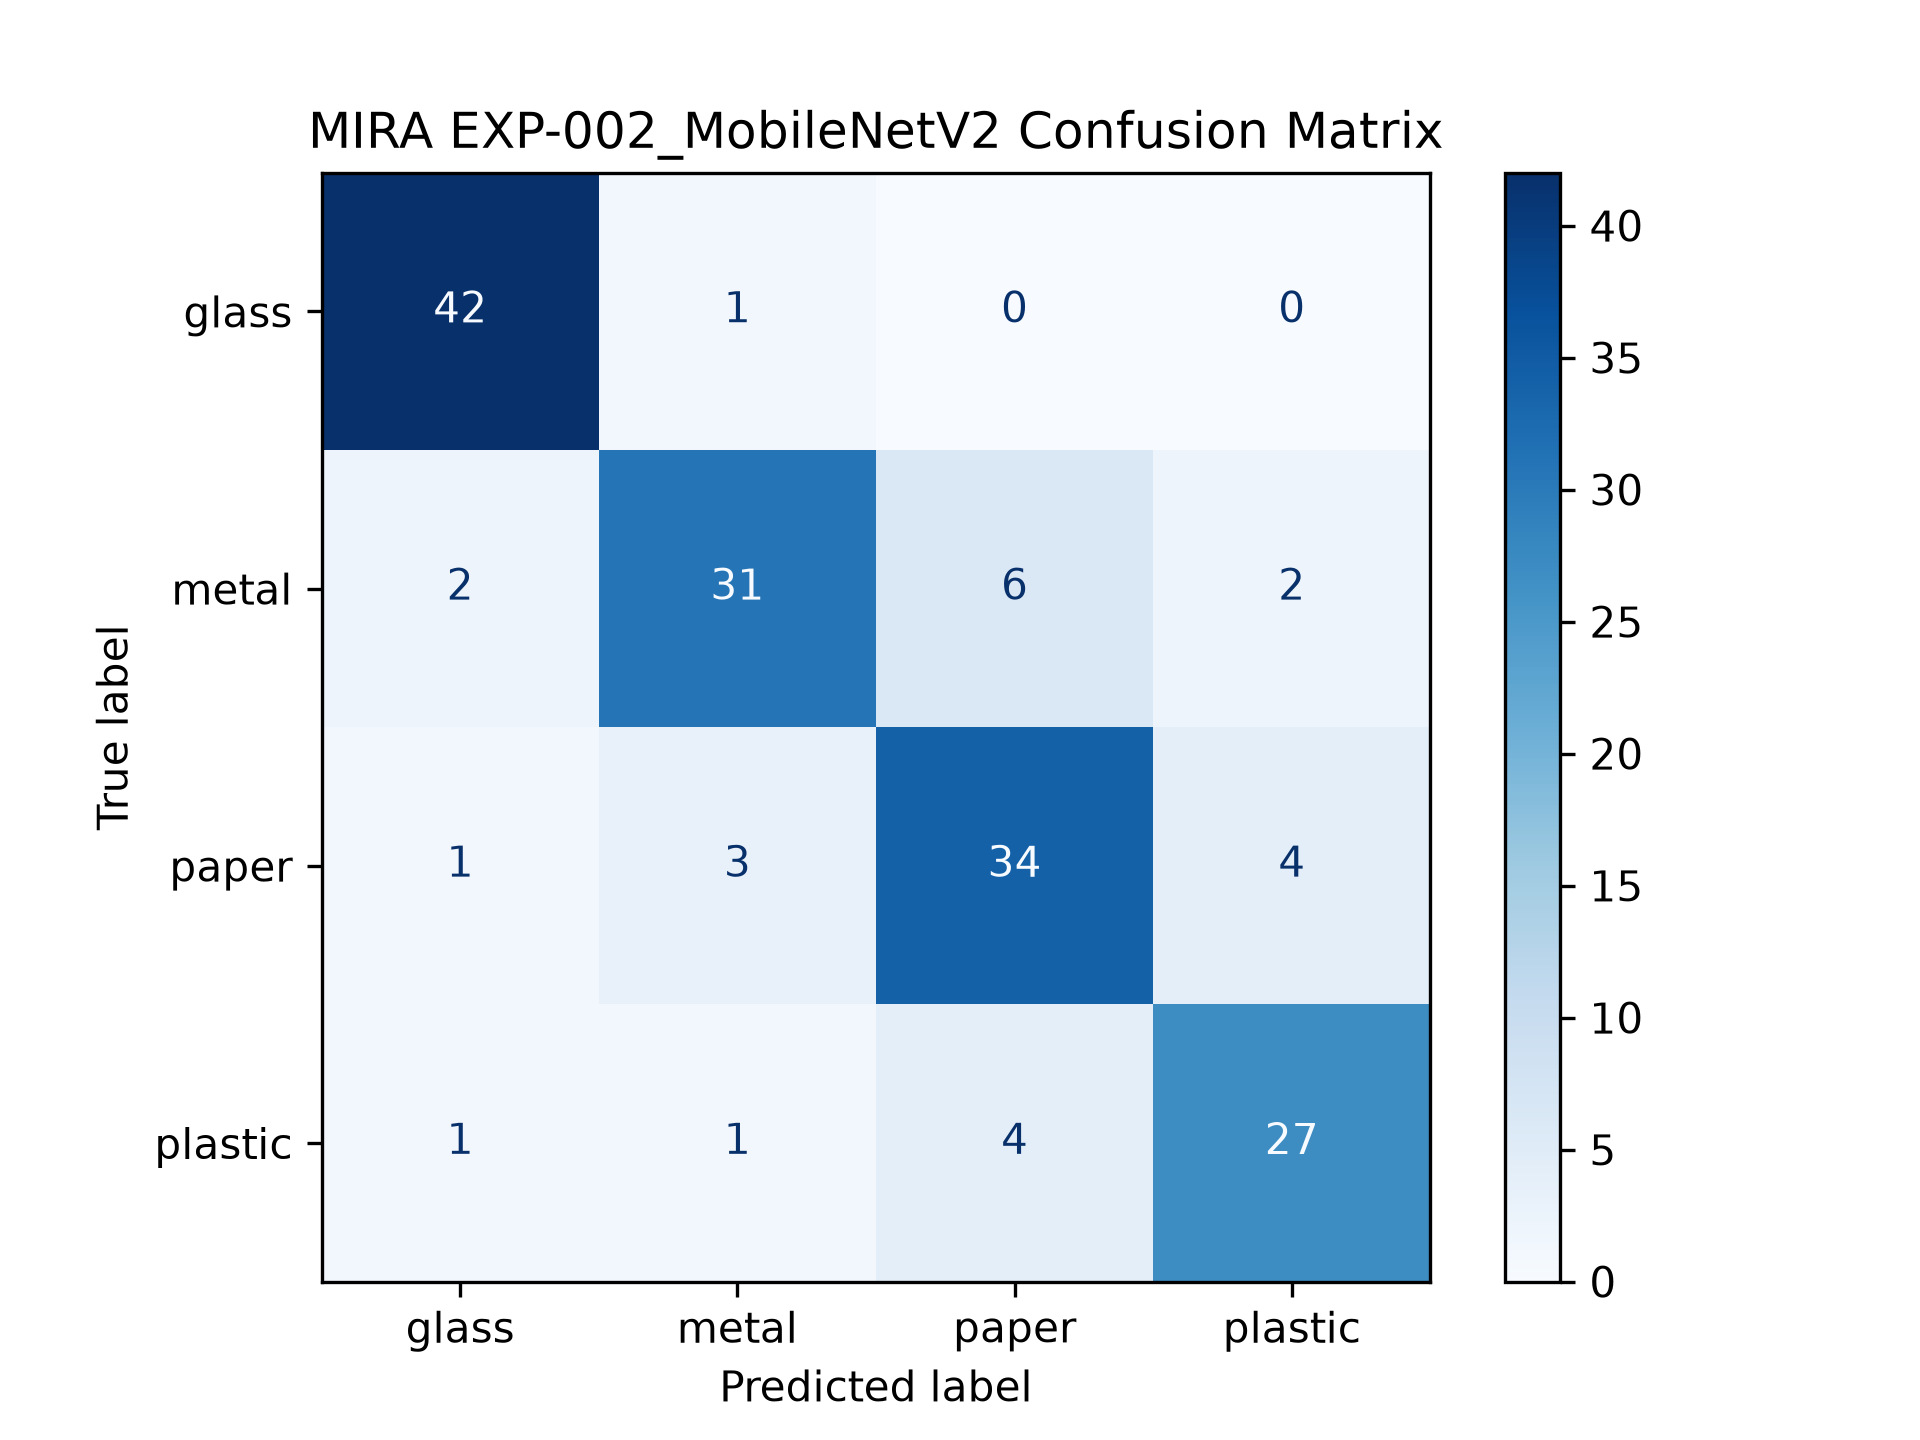
\includegraphics[width=\textwidth, keepaspectratio]{figures/exp2-confusion.png}
        \caption{EXP-002 (Frozen)}
    \end{subfigure}
    \hfill
    \begin{subfigure}[b]{0.31\textwidth}
        \centering
        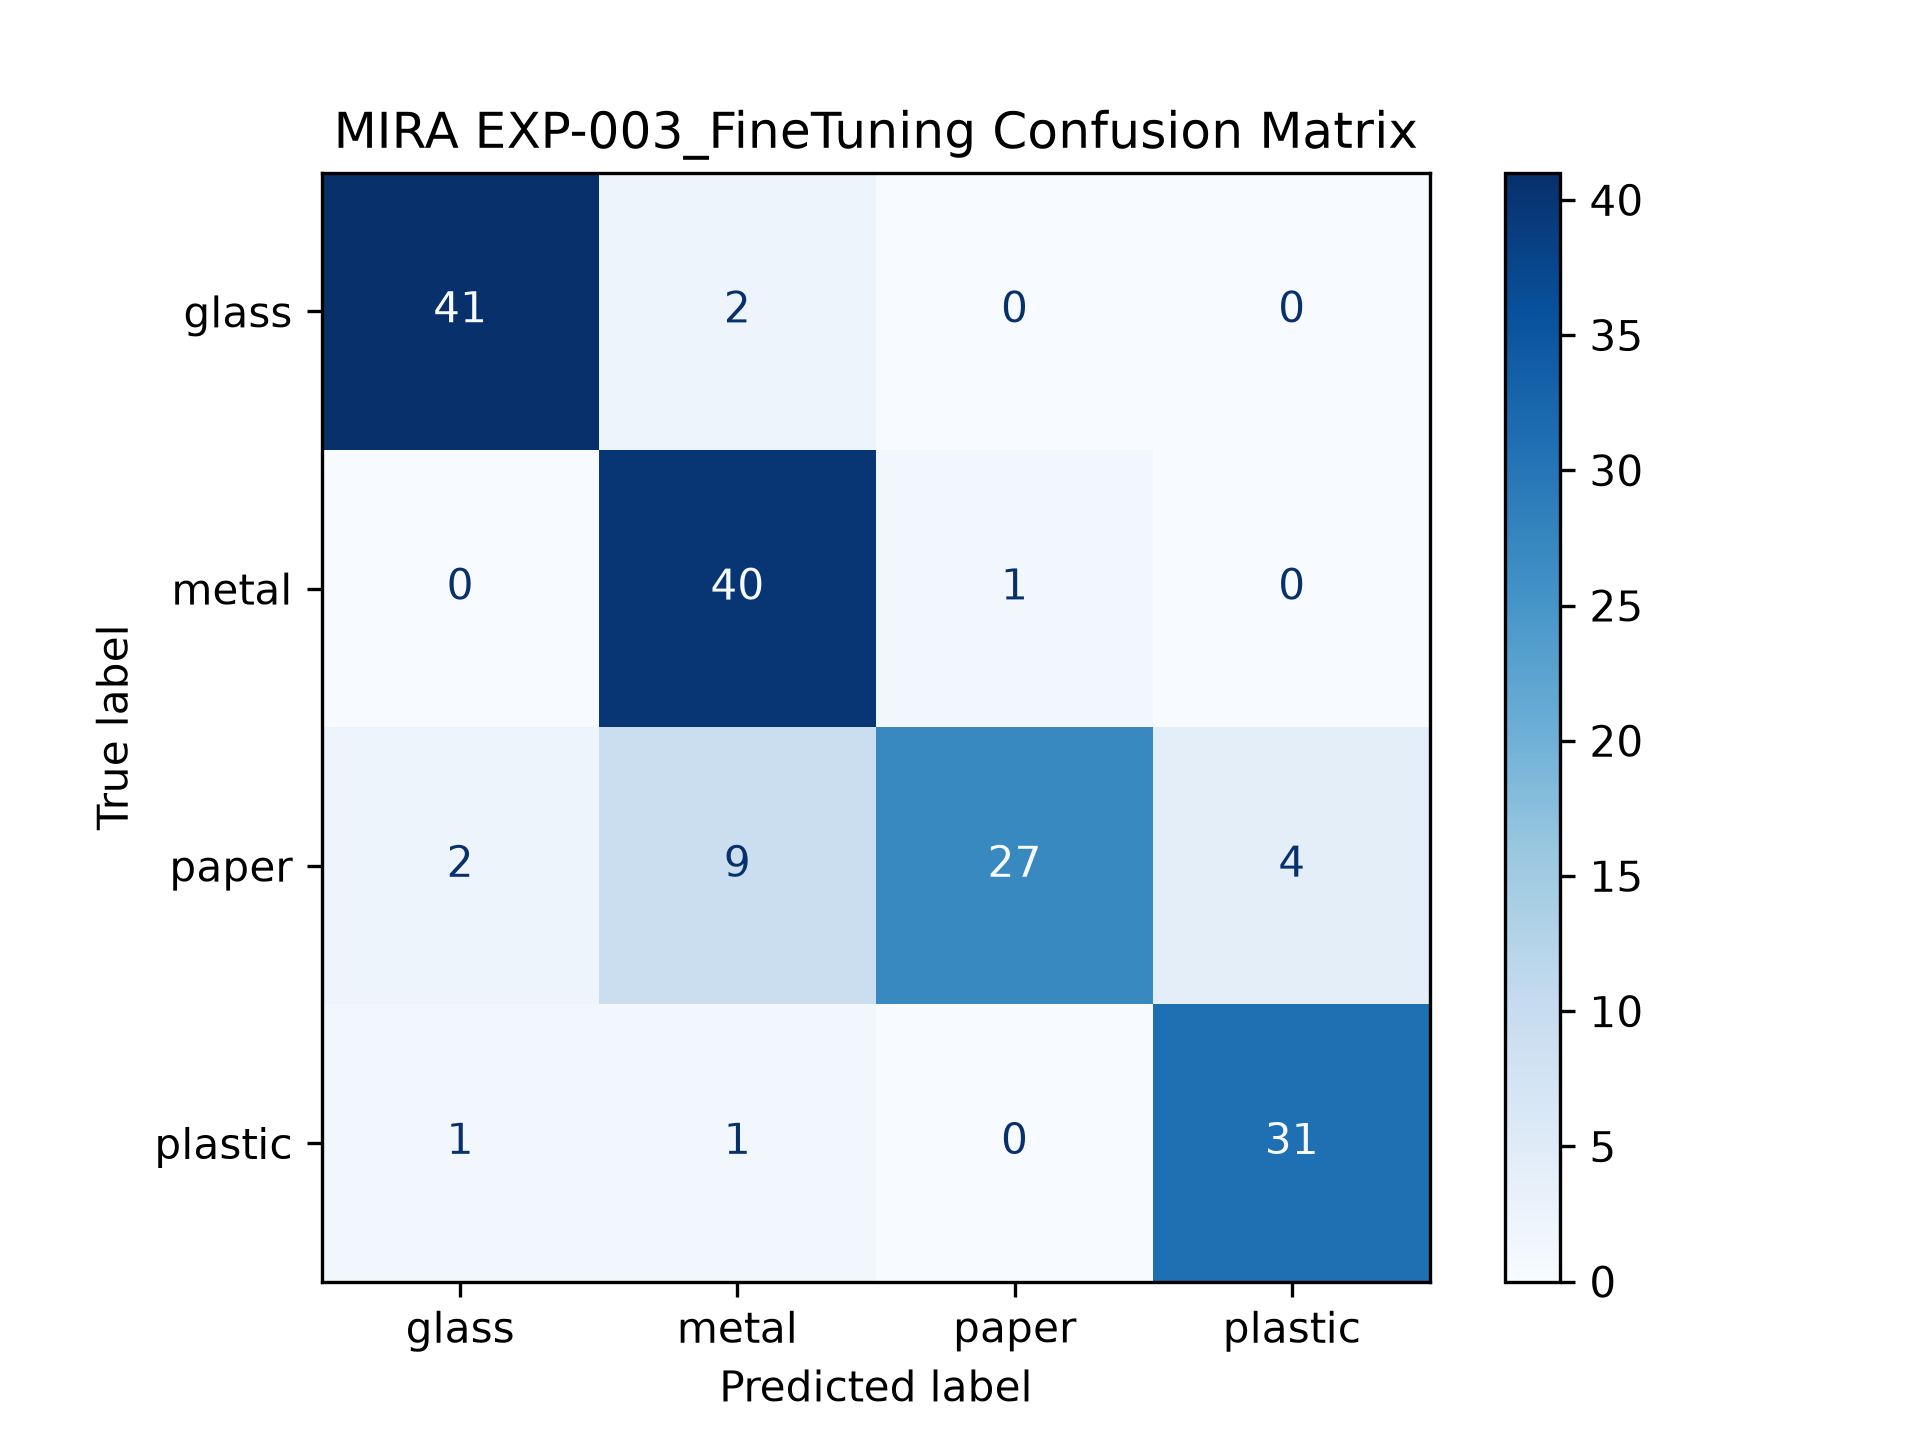
\includegraphics[width=\textwidth, keepaspectratio]{figures/exp3-confusion.png}
        \caption{EXP-003 (Fine-Tune)}
    \end{subfigure}
    \caption{Confusion Matrices der drei Klassifikationsmodelle. Im EXP-001 werden Papier und Metall stark als Plastik fehlklassifiziert. EXP-003 reduziert diese systematischen Fehler deutlich.}
    \label{fig:conf-class}
\end{figure}

\subsection{Quantisierung (EXP-004)}
Das beste Keras-Modell (EXP-003) wurde per TensorFlow Lite exportiert. Dabei wurden ein FP32-Modell und anschließend ein voll quantisiertes INT8-Modell erzeugt. Für die Kalibrierung kam eine repräsentative Stichprobe von 100 Bildern zum Einsatz \cite{deng2020model}. Die Klassifikationsleistung blieb dabei nahezu identisch (\SI{87.35}{\percent} vs.\ \SI{87.42}{\percent} des FP32-Modells), während die Modellgröße um den Faktor 9 auf \SI{2.61}{\mega\byte} sank.

\subsection{Detektionsphase YOLOv8 (EXP-005 bis EXP-009)}
Die zweite Projektphase drehte sich um Objekterkennung. Zunächst wurde ein YOLOv8-Nano-Modell auf einem einfachen Benchmark trainiert (EXP-005). Dieses Modell erreichte zwar eine scheinbar hohe Validierungsgenauigkeit von \SI{82.3}{\percent} mAP50. Diese hohe Metrik erwies sich jedoch bei einer detaillierten Fehleranalyse als Artefakt eines extremen Hintergrund-Overfittings (Background Leakage): Da der Canny-Edge-Auto-Labeler die kontrastreichen Kanten und Helligkeitsgradienten des Schreibtischrahmens umschloss, lernte das Netzwerk nicht die Müllobjektspezifika selbst, sondern korrelierte die Geometrie der gesamten Arbeitsfläche mit der Zielklasse. Dies erklärt die hohe Genauigkeit auf dem monotonen Test-Set der Tischoberfläche, führte aber zu einem vollständigen Versagen (mAP50 nahe \SI{0}{\percent}) bei Tests auf abweichenden Hintergründen. Dieser GIGO-Effekt (Abschnitt~\ref{sec:method-gigo}) zwang zur Verfeinerung der Datengrundlage. Spätere Modelle (EXP-006, EXP-009) trainierten auf gemischten Wild-Datensätzen und dem bereinigten TrashNet-Datensatz \cite{yang2016classification}.

\begin{figure}[H]
    \centering
    \begin{subfigure}[b]{0.48\textwidth}
        \centering
        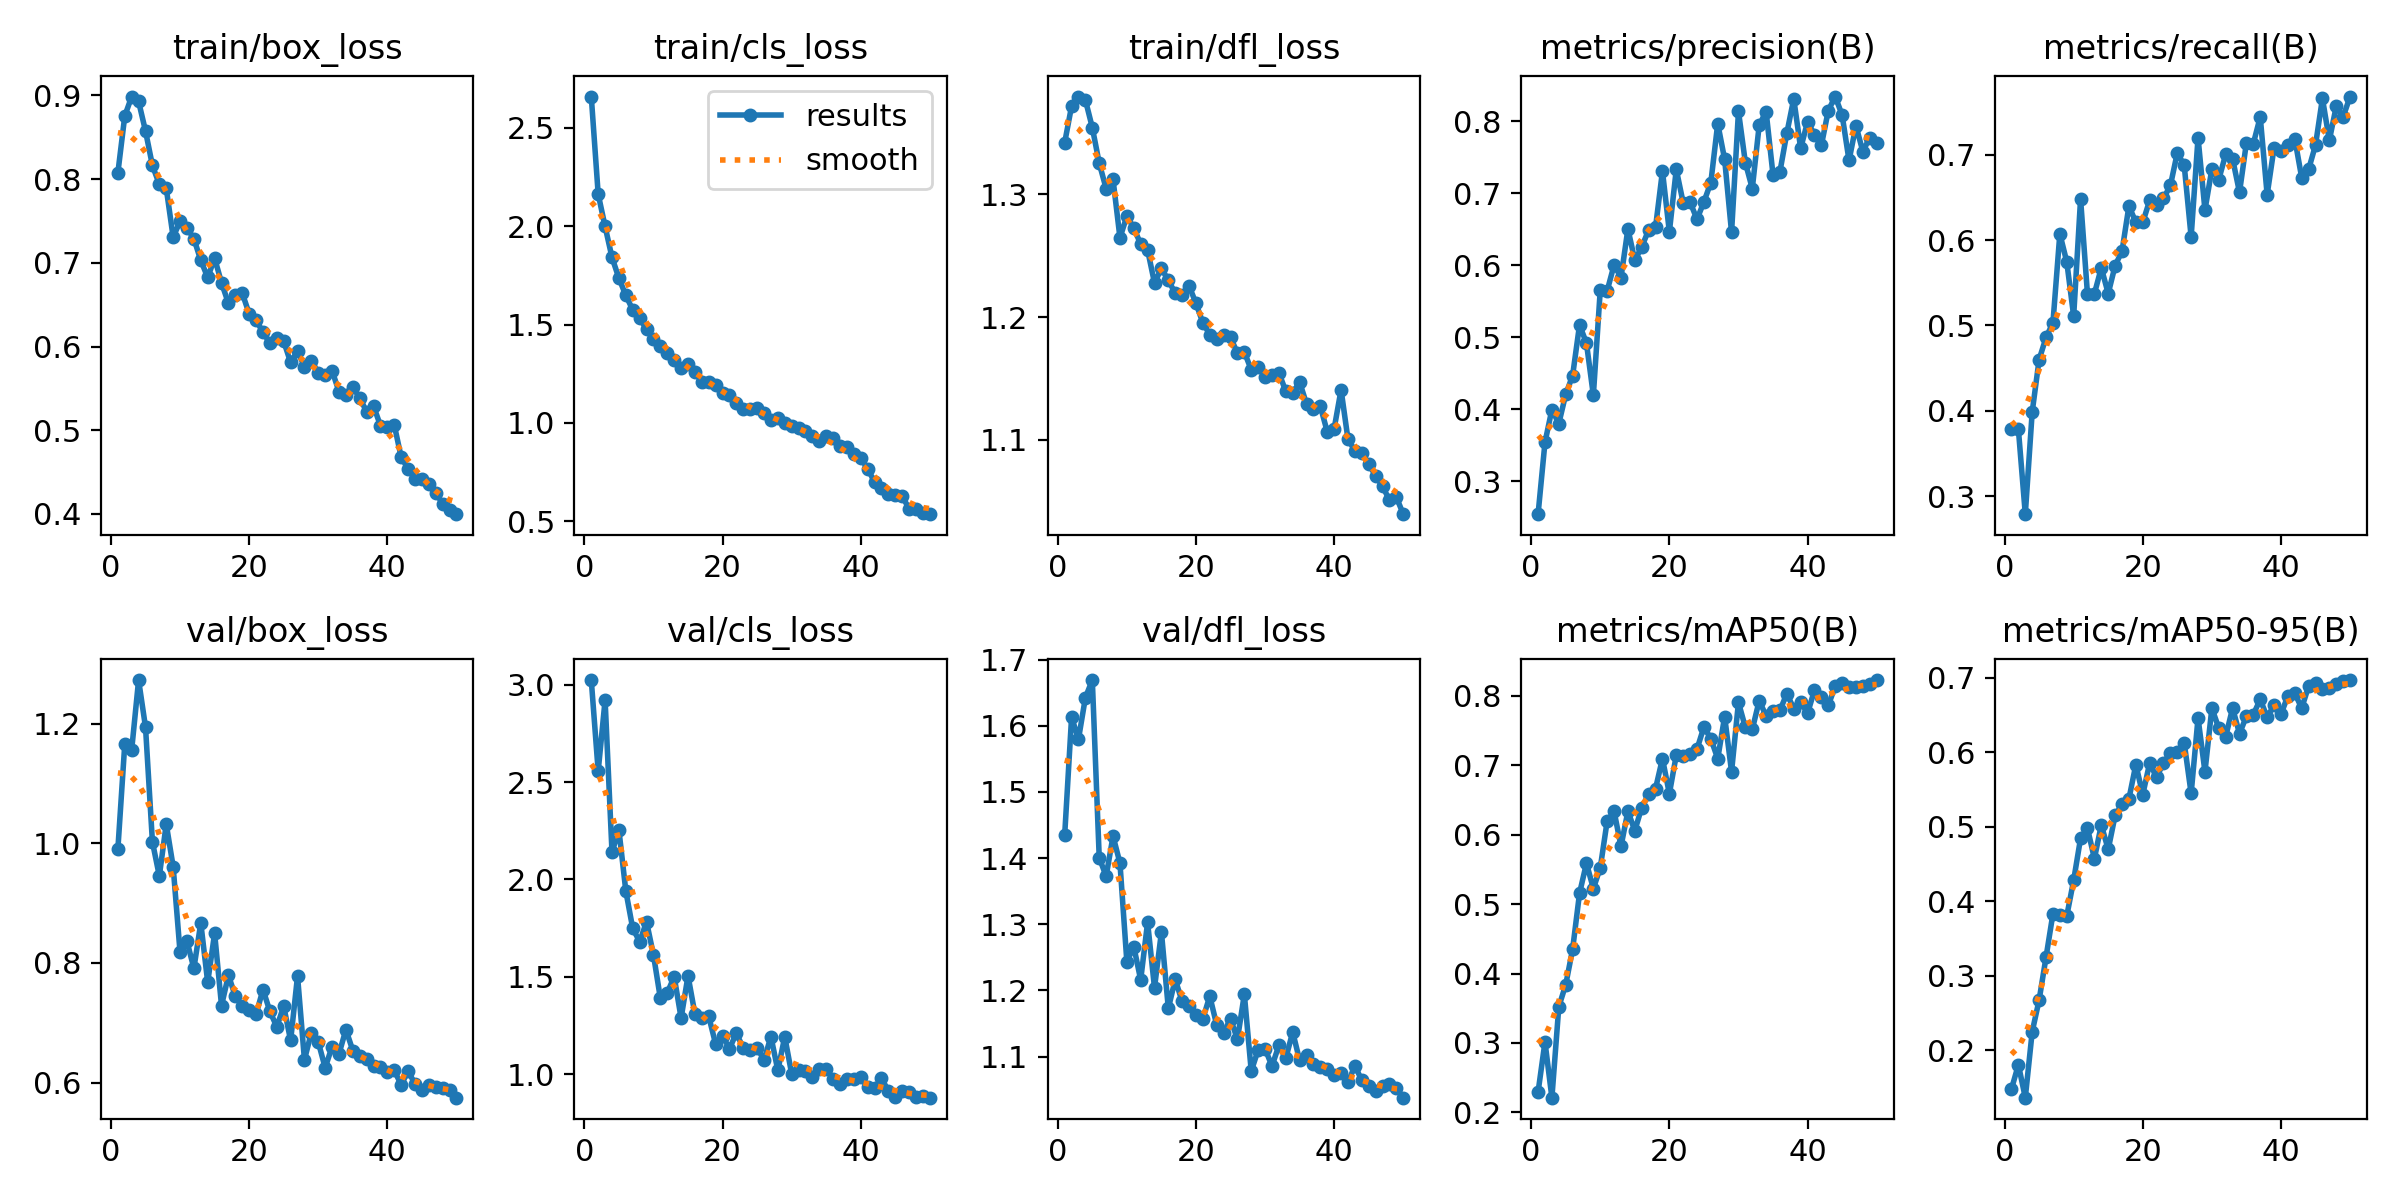
\includegraphics[width=\textwidth, keepaspectratio]{figures/yolov8-results.png}
        \caption{Trainingsmetriken (EXP-009)}
    \end{subfigure}
    \hfill
    \begin{subfigure}[b]{0.48\textwidth}
        \centering
        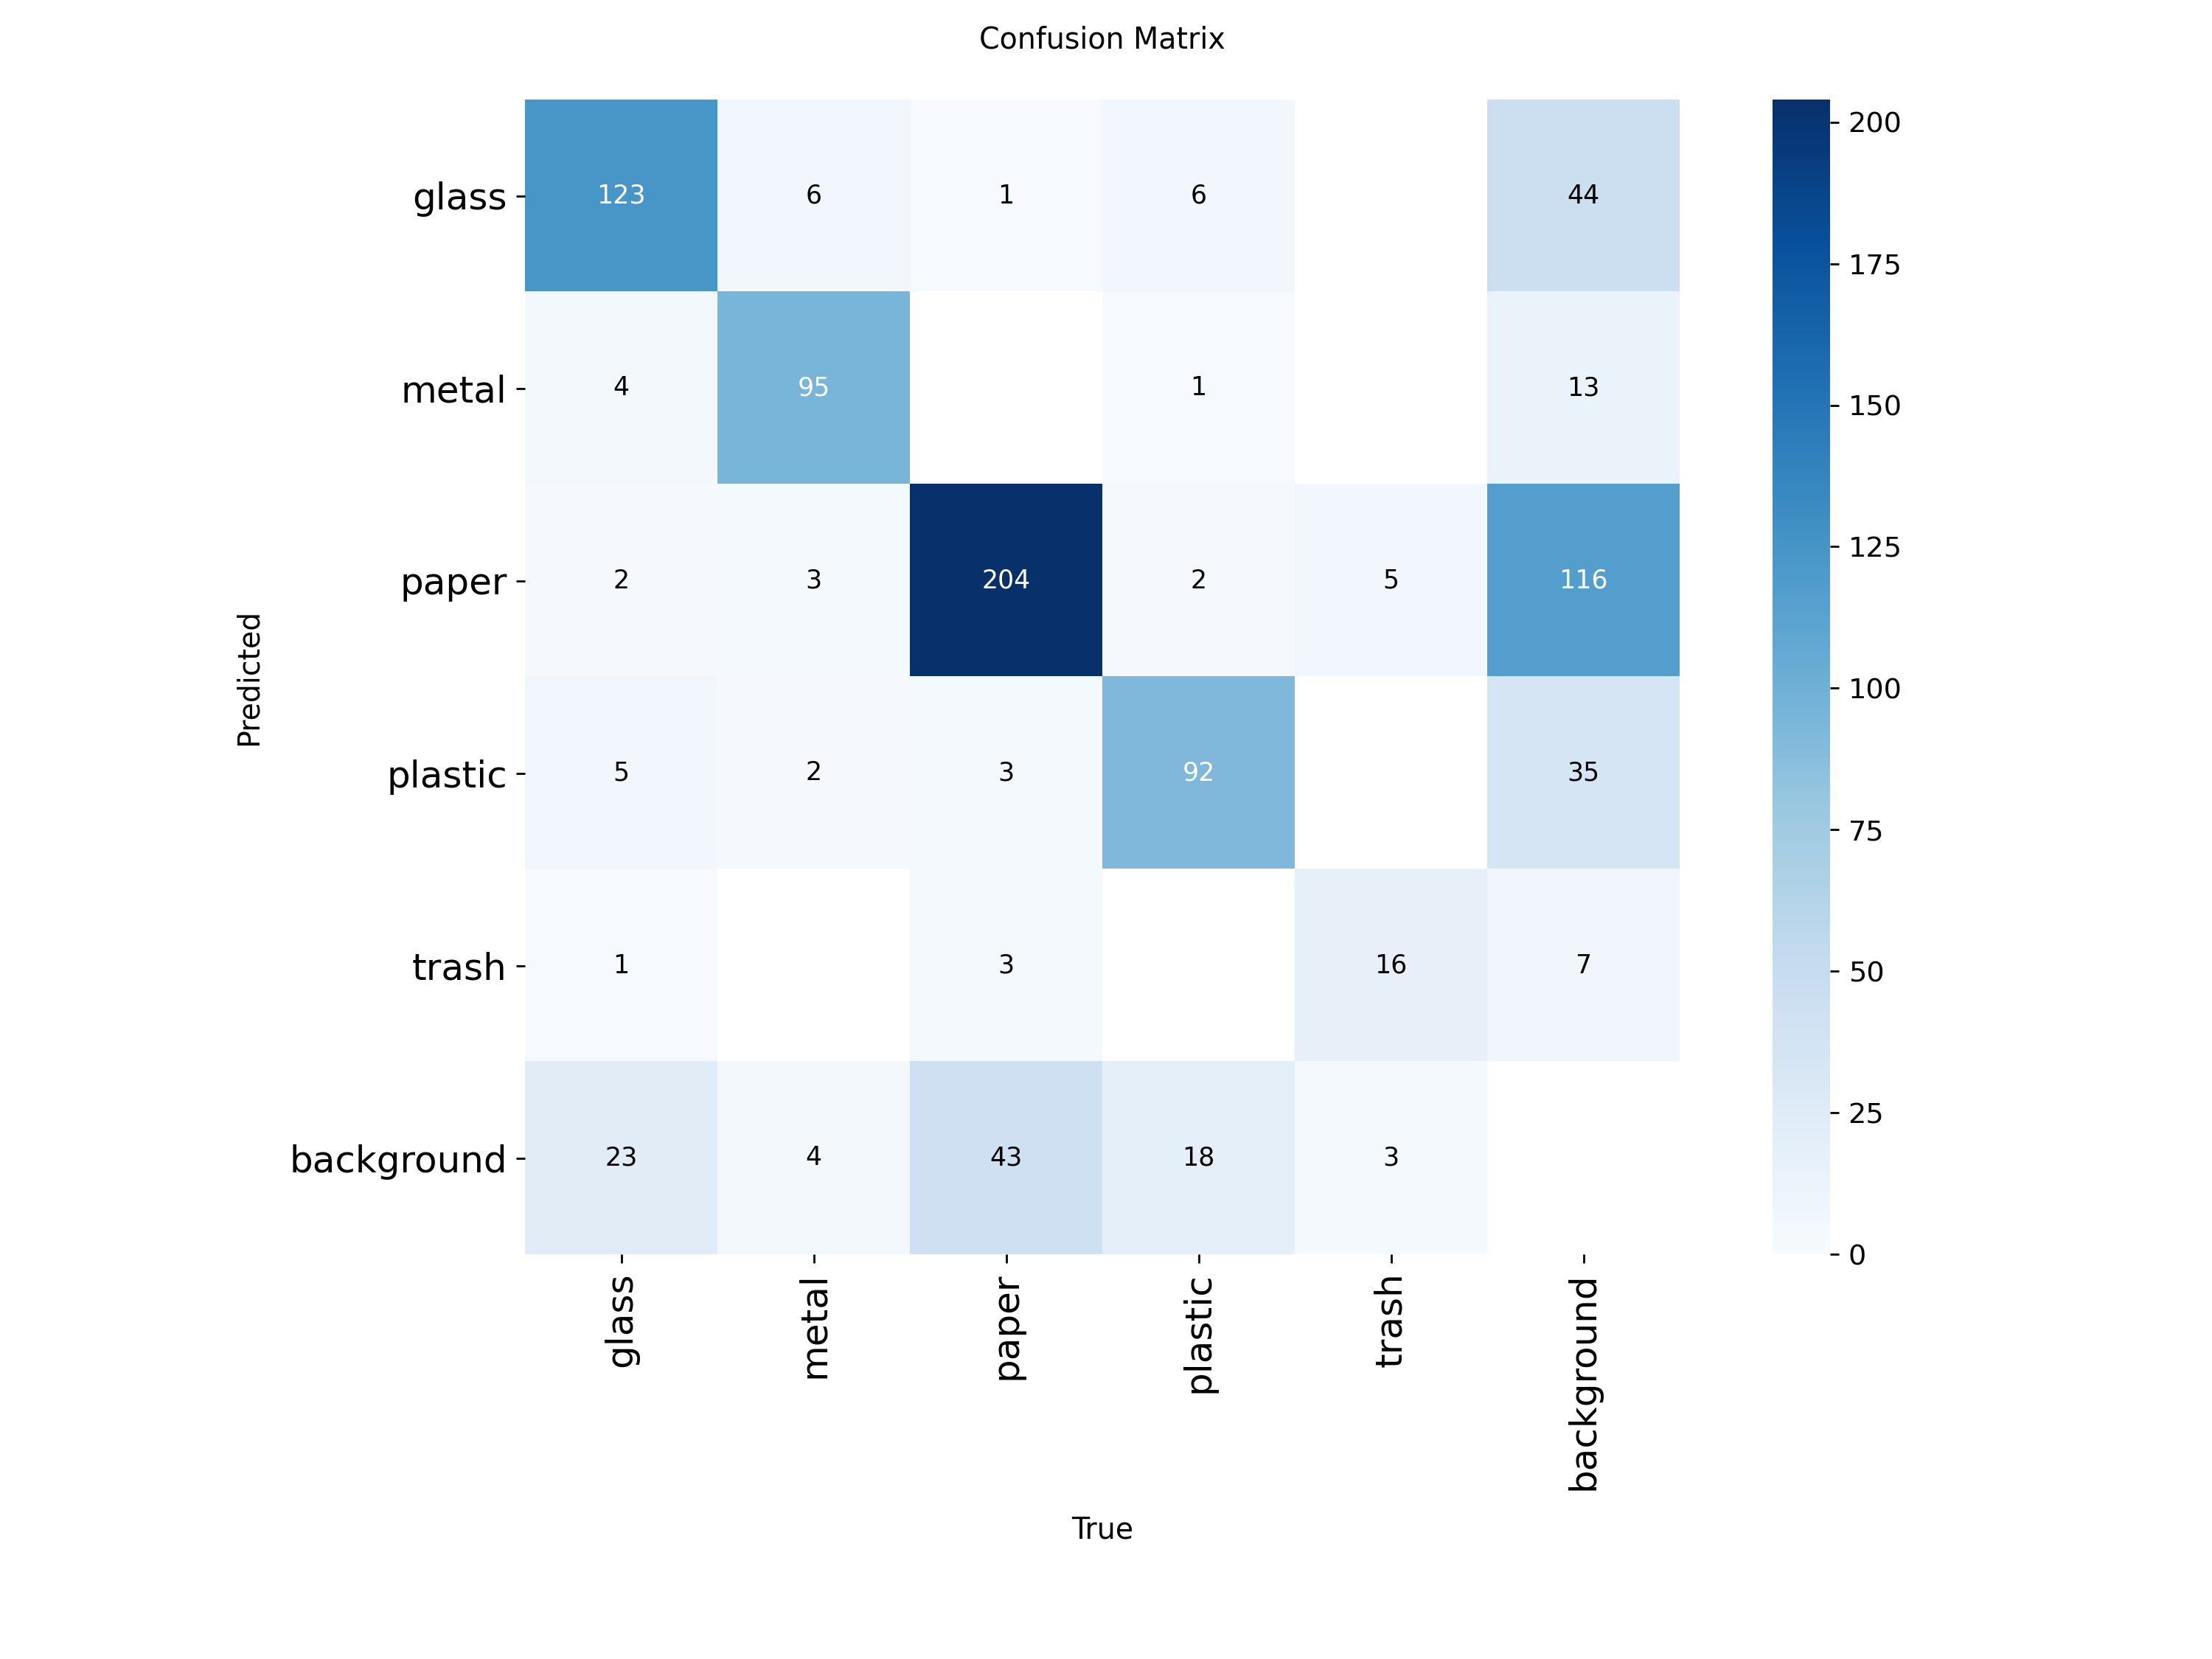
\includegraphics[width=\textwidth, keepaspectratio]{figures/yolov8-confusion.png}
        \caption{Konfusionsmatrix (EXP-009)}
    \end{subfigure}
    \caption{Ergebnisse des YOLOv8-Nano-Detektors (Pristine TrashNet, EXP-009). mAP50 konvergiert auf \SI{72.8}{\percent}; Hintergrund-Fehlklassifikationen sind das dominierende Fehlermuster.}
    \label{fig:yolo}
\end{figure}

\subsection{Architekturmigration: YOLO11n (EXP-013 bis EXP-016)}
\label{sec:exp-yolo11}
Im dritten Abschnitt der Detektionsphase wurde die Basisarchitektur von YOLOv8-Nano (\SI{3.01}{Mio.}\ Parameter) auf YOLO11n (\SI{2.58}{Mio.}\ Parameter) migriert \cite{ultralyticsyolov8}. YOLO11n ist kompakter (6,3 GFLOPs) und erreicht auf dem fusionierten mira\_v2-Datensatz (\num{4024} Bilder, TACO + TrashNet) einen ausgeglichenen mAP50 von \SI{55.1}{\percent} (EXP-013). Ein systematischer Vergleich evaluierte anschließend den Einfluss zusätzlicher Datenquellen:

\begin{itemize}
    \item \textbf{EXP-013 (Baseline):} TACO~\cite{proenca2020taco} + TrashNet~\cite{yang2016classification} (\num{4024}~Bilder) $\rightarrow$ mAP50~\SI{55.1}{\percent}
    \item \textbf{EXP-014 (+Roboflow):} Zusätzlich Roboflow Trash Detection \cite{roboflow2023trash} $\rightarrow$ mAP50~\SI{60.7}{\percent} \textbf{(Bestes Modell)}
    \item \textbf{EXP-015 (+WaRP):} Roboflow ersetzt durch WaRP~Waste~Detection \cite{warp2024dataset} $\rightarrow$ mAP50~\SI{56.0}{\percent}
    \item \textbf{EXP-016 (WaRP-only):} Ausschließlich WaRP $\rightarrow$ mAP50~\SI{58.8}{\percent} (jedoch ohne \textit{trash}-Klasse)
\end{itemize}

EXP-014 erzielt den besten Gesamtmittelwert (+5,6~pp über EXP-013), mit besonders starken Zuwächsen bei Trash (+11,3~pp) und Glass (+6,3~pp). Der WaRP-Datensatz (EXP-015) verbessert Glass signifikant (+24,8~pp), senkt aber Trash drastisch (−12,6~pp), da WaRP keine Trash-Klasse enthält. EXP-016 (WaRP-only) erreicht ohne Trash-Klasse \SI{58.8}{\percent} mAP50 bei starken Glass-Ergebnissen (\SI{77.7}{\percent}). Die Ergebnisse des finalen Fusionsmodells EXP-014 sind in Abbildung \ref{fig:yolo11n} dargestellt, der vollständige Modellvergleich in Abbildung \ref{fig:heatmap-4datasets}.

\begin{figure}[H]
    \centering
    \begin{subfigure}[b]{0.48\textwidth}
        \centering
        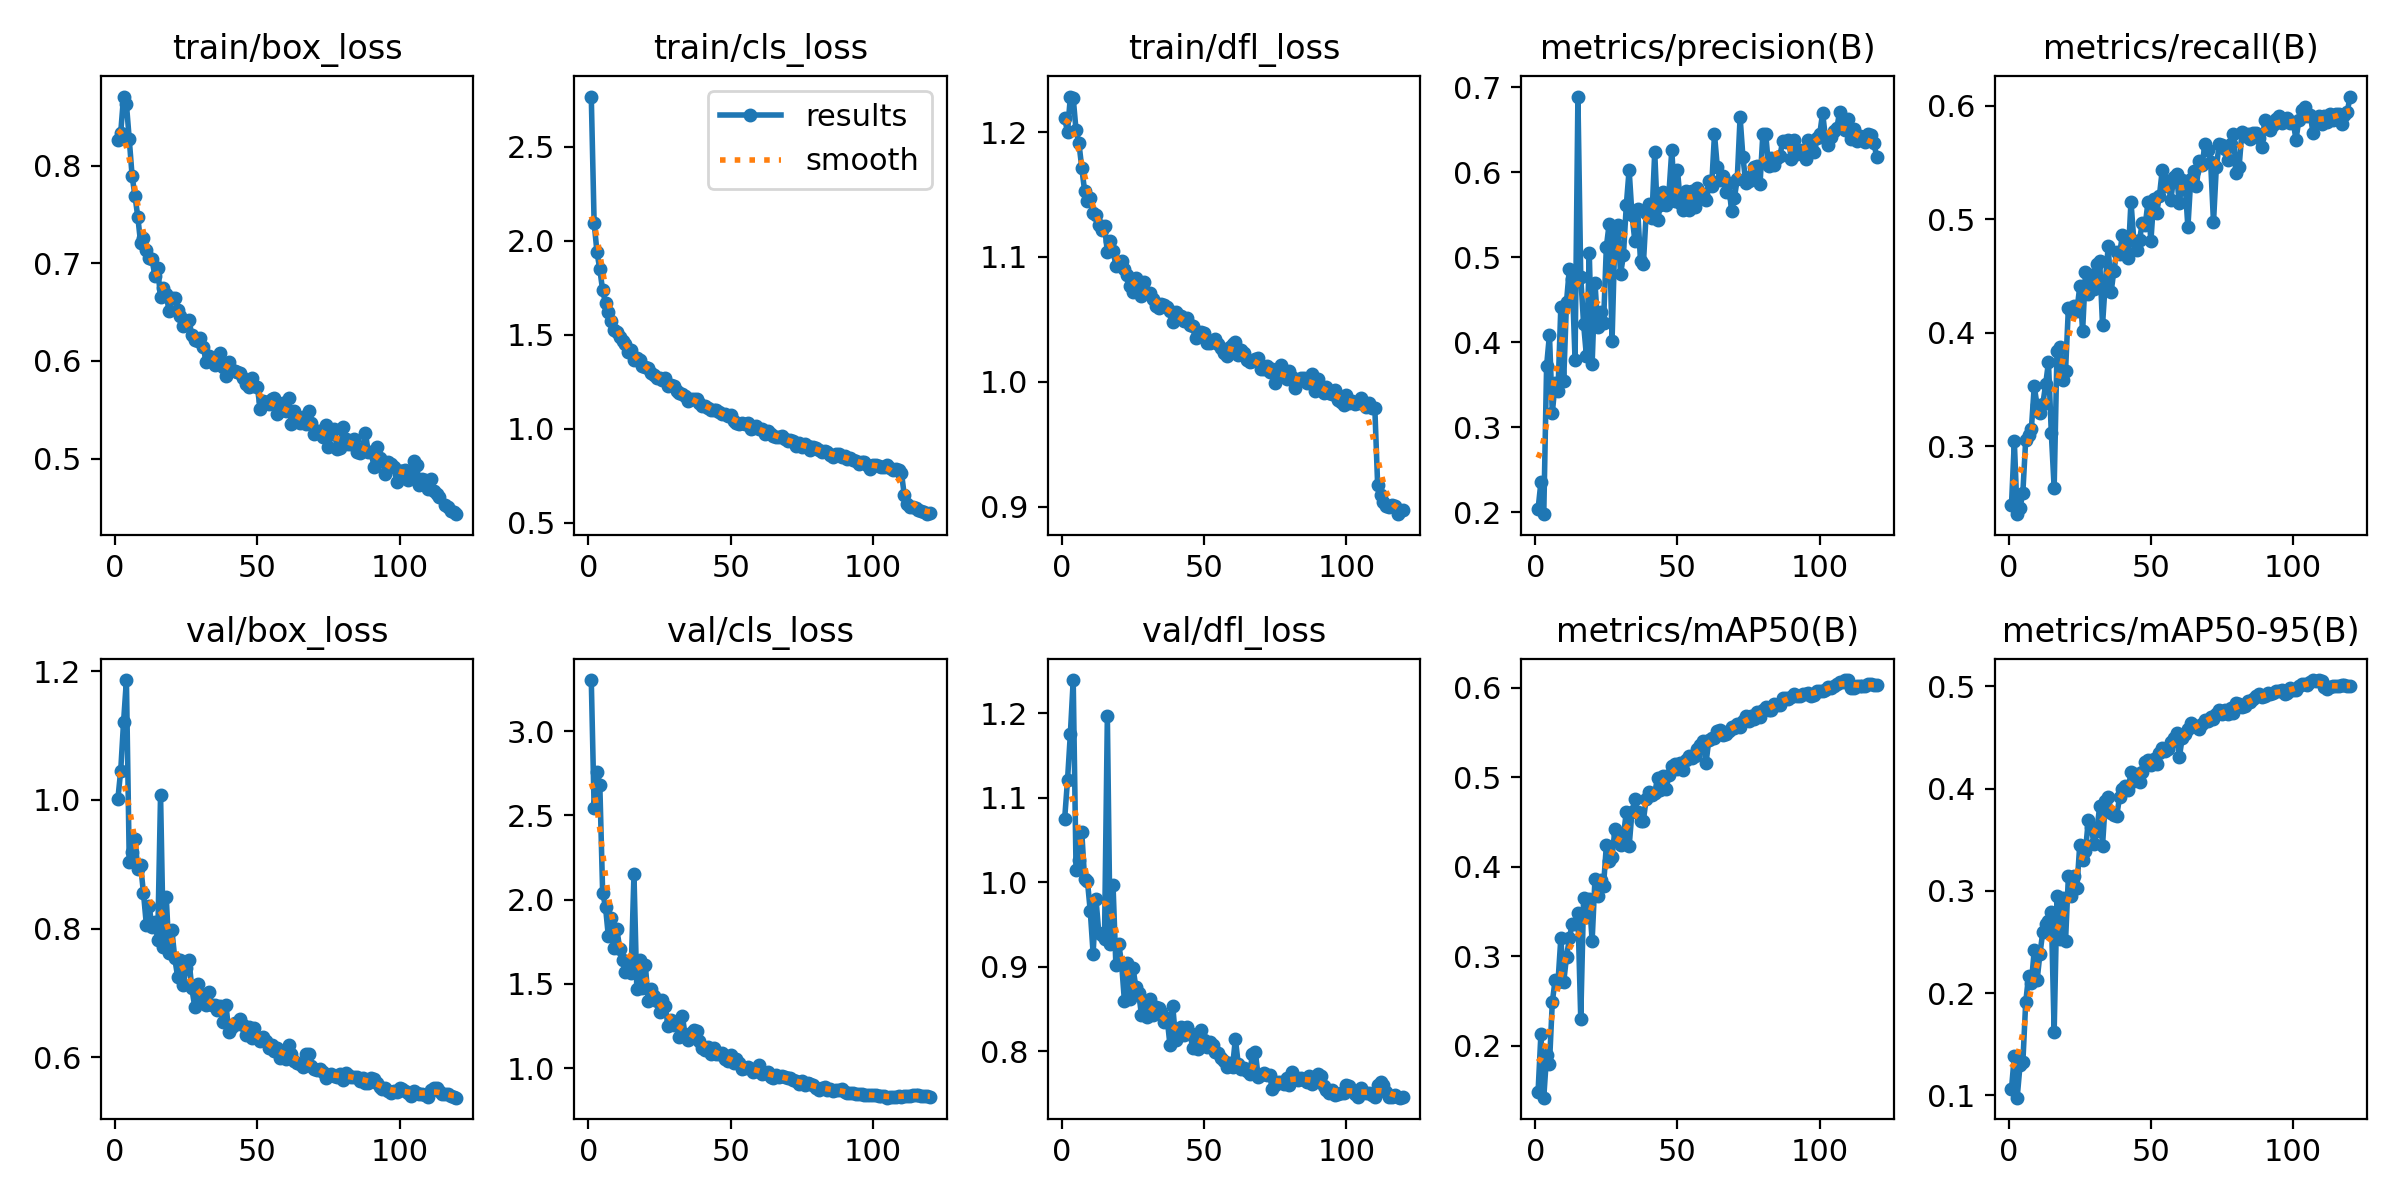
\includegraphics[width=\textwidth, keepaspectratio]{figures/exp14-results.png}
        \caption{Trainingsmetriken (EXP-014)}
    \end{subfigure}
    \hfill
    \begin{subfigure}[b]{0.48\textwidth}
        \centering
        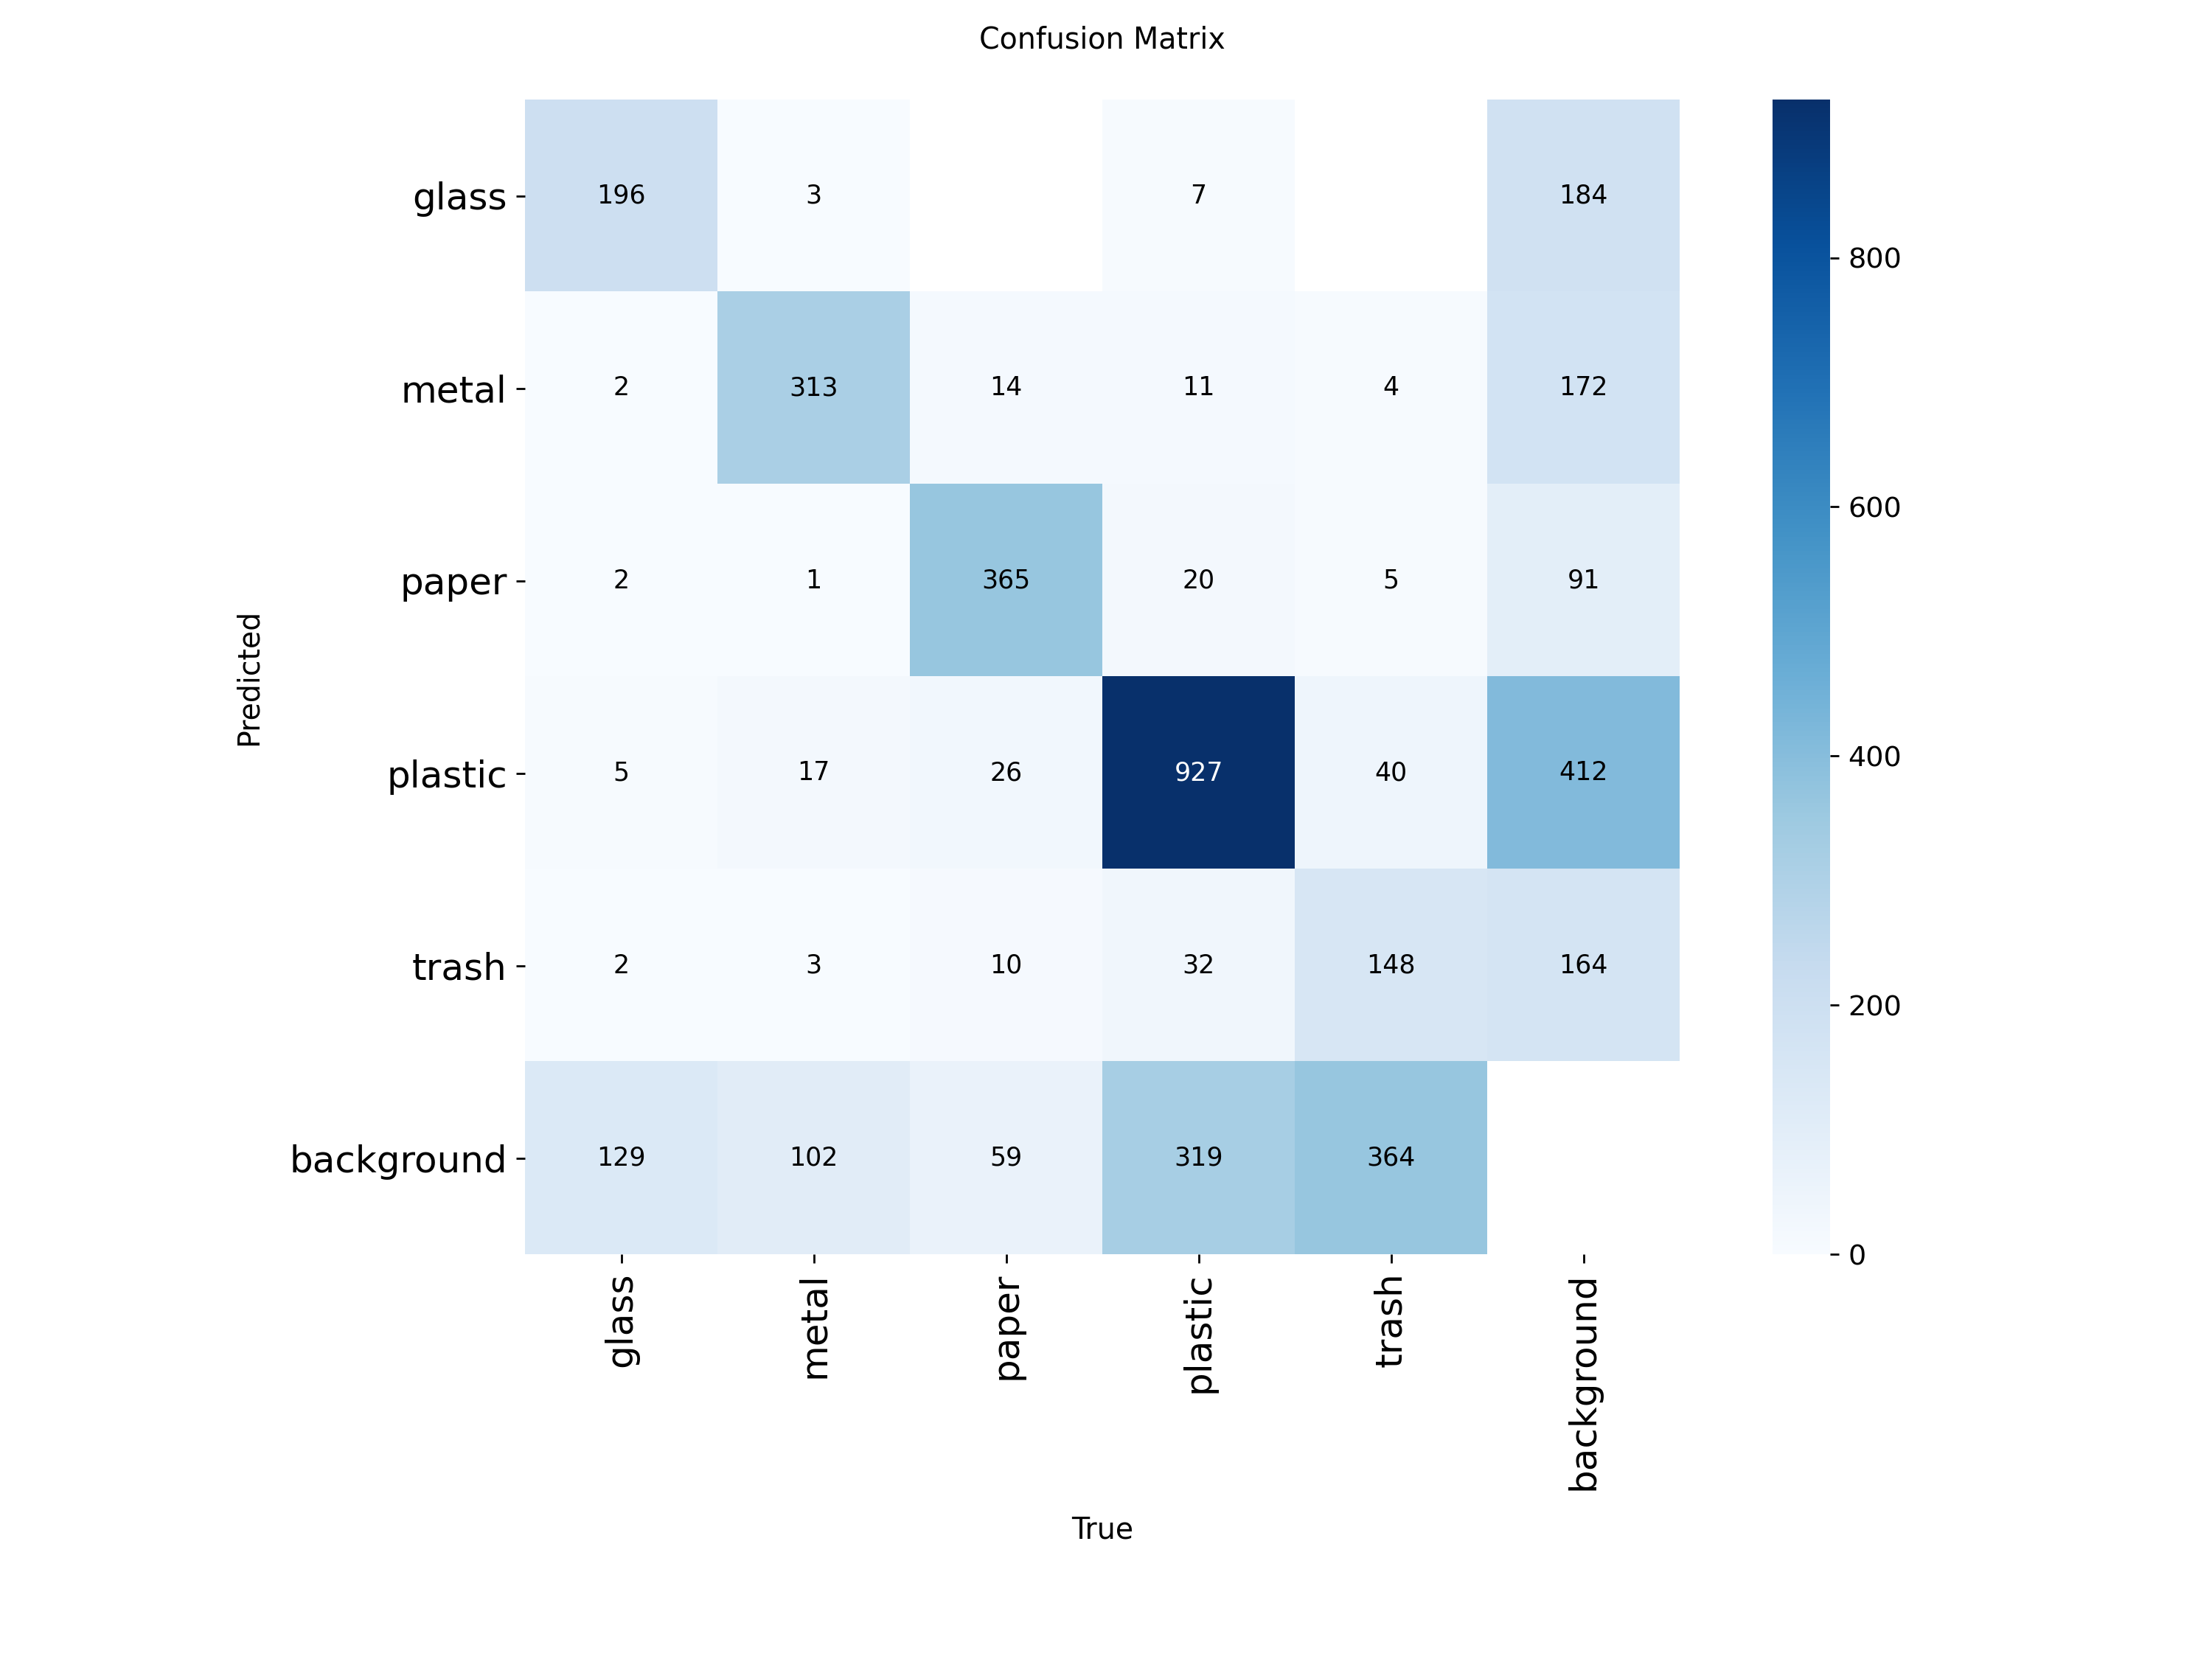
\includegraphics[width=\textwidth, keepaspectratio]{figures/exp14-confusion.png}
        \caption{Konfusionsmatrix (EXP-014)}
    \end{subfigure}
    \caption{Ergebnisse des besten YOLO11n-Detektors (EXP-014). Durch die Datenfusion aus TACO, TrashNet und Roboflow wird ein robuster mAP50 von \SI{60.7}{\percent} erreicht.}
    \label{fig:yolo11n}
\end{figure}